% Chapter 7
\chapter{Conclusions}\label{Chapter7}
The work that covers the  fiducial cross section measurements of the Higgs boson production  in the $H \rightarrow 4\ell$  decay channel ($\ell = e, \mu$) in proton-proton 
collisions at $\sqrt{s}=7, 8, 13$~TeV is presented in this dissertation. These measurements helps to probe the structure, nature
of interaction of Higgs boson  with decaying particles. These measurements provide a direct probe into SM Higgs sector perturbative QCD  calculations at the TeV 
energy scale. Any deviation of integrated or differential distributions from SM expectations would  provide a direct hint to BSM contributions.
The differential  distributions has been extracted only for 8~TeV dataset due to limited statistics of 7 and 13~TeV dataset. 
\par These measurements  are made using data from pp collisions corresponding to integrated 
luminosities of \usedLumiA, \usedLumiB  and 2.8~\ifb  at $\sqrt{s}=7$, 8 and 13~TeV. To minimize the dependence of the results on the 
underlying model of the Higgs boson production  mechanism and  its properties, the cross sections are extracted in a fiducial phase space closely matching
with the experimental acceptance. The remaining model dependence is extracted by repeating the measurement for SM and other exotic model and reported as 
a distinct systematic uncertainty. All measurements include the correction for the finite detection
efficiency and resolution effects. As $\sigma \times BR$ strongly depend upon Higgs mass, the measurement has been extracted assuming $m_H =  125.0$~GeV, as
measured using the $H \rightarrow 2\gamma$ and $H \rightarrow 4\ell$ decay channels by the CMS experiment~\cite{Reference39}. 

The differential fiducial cross sections are also presented using the  8~\TeV~data as a function several kinematic observables which are sensitive to the
Higgs-boson  production mechanisms: rapidity and transverse momentum of the four-lepton 
system, associated jet multiplicity, transverse momentum of the leading jet and separation between the leading jet and the Higgs boson candidate. 
The results are also reported for kinematic observables which are sensitive to the Higgs boson decay mechanisms: the invariant masses of the two 
lepton pairs and five helicity angles formed by the leptons in the Collins-Soper frame~\cite{Reference40}.
The integrated fiducial cross sections are measured to be  $0.56^{\rm +0.67}_{\rm -0.44}({\rm stat.})^{\rm +0.21}_{\rm -0.06}({\rm sys.}) ^{+0.02}_{-0.02}({\rm model}){\rm fb}$,
$1.11^{\rm +0.41}_{\rm -0.35}({\rm stat.)^{\rm +0.14}_{\rm -0.10}({\rm sys.}) ^{+0.08}_{-0.02}({\rm model}){\rm fb}$
and $2.48^{+1.45}_{-1.12}({\rm stat.})^{+0.28}_{-0.17}({\rm sys.})^{+0.01}_{-0.04}({\rm model})~{\rm fb}$ at 7, 8 and 13\TeV~respectively.

\par 
 Measurements of the integrated cross section of Z boson production in the $Z \rightarrow 4\ell$ decay channel, as well as its ratio
to the $\Hllll$ fiducial cross section, have also been performed using the 8~TeV collision data. The differential fiducial cross section  of
$Z \rightarrow 4\ell$ has been performed on the footings of Higgs measurement, using same differential variables
and bins using  8~TeV data.
The integrated Z boson production cross section measurement using $Z \rightarrow 4\ell$ decay channel at 7~TeV has already been measured in 
Ref.~\cite{Z4LPaper}. The integrated ratio of $H\rightarrow4\ell$ and $Z\rightarrow4\ell$ fiducial cross section is also reported 8~TeV data. The motivation
for the ratio is to cancel out systematic uncertainties and to validate Higgs measurements. The integrated fiducial cross section for the Z boson production in  
the $Z \rightarrow 4\ell$ decay channel is measured to be $4.81^{\rm +0.69}_{\rm -0.63} \, {\rm(stat.)}\, ^{\rm +0.18}_{\rm -0.19}\,  {\rm (sys.)}$. Ratio of 
integrated fiducial cross section of H$\rightarrow 4l$ and Z$\rightarrow 4l$ measured to 
be  $0.21^{\rm +0.09}_{\rm -0.07} \, {\rm(stat.)}\, ^{\rm +0.01}_{\rm -0.01}\,  {\rm (sys.)}$.
\par 
 All results have been corrected for the detection efficiency and resolution  effects to allow for direct comparison with the SM predictions. The agreement between 
 SM predictions and measured $H\rightarrow4\ell$ cross section measurement at $\Sqrt{s} = $7, 8, 13~TeV is found be good. These model independent cross
 section measurements can be compared with any theoretical predictions in future with better accuracy. As these results are statistically limited so more 
 data at $\sqrt{s} = 13$~TeV will allow better discrimination between measurements and theoretical predictions. The results $Z \rightarrow 4\ell$ and 
 ratio of integrated fiducial cross section of H$\rightarrow 4l$ and Z$\rightarrow 4l$ also find to be consistent with SM.

\chapter{Outlook}\label{Chapter8}
After the discovery of the Higgs boson, it became very natural and important to measure Higgs boson properties as precise as possible. Precision measurements of 
the Higgs boson properties can provide us direct or indirect hint  of any new physics for which we are looking desperately. This dissertation presented the 
measurements of integrated and differential Higgs boson via $H \to 4\ell$ decay channel which is an important Higgs boson property.  $\Z \to 4\ell$  decay channel
is also important to test SM prediction and to validate the methodology  of $H \to 4\ell$. These measurements provide a direct probe into SM Higgs sector 
perturbative QCD  calculations at the TeV energy scale. Any deviation of integrated or differential distributions from SM expectations would  provide a direct
hint to BSM contributions. The differential  distributions has been extracted only for 8~TeV dataset due to limited statistics of 7 and 13~TeV dataset. These 
differential distributions are sensitive gluon fusion production mechanism, PDFs of  colliding proton, theoretical modeling of hard quark radiation and relative 
contribution of different Higgs boson production mechanism. The measurement of the ratio  of $H\rightarrow4\ell$ and $Z\rightarrow4\ell$ has also been performed, where the masses
of both resonance are allowed to float and fit for difference of masses of both resonances $\Delta m = m_H - m_Z$ and the Higgs boson $m_H$. This 
scenario helps to reduce the systematic uncertainty due to lepton momentum scale resolution which would also be useful for RunII for Higgs mass measurements.

\par

The current measurements are dominated by statistical uncertainties. The studies based on simulations
showed that the uncertainties on Higgs cross section measurements with 100~\fbinv pp collisions data would be almost equal to the current theoretical uncertainties 
as shown in Figure~\ref{fig:Higgs_XS_100}. The Figure~\ref{fig:Higgs_XS_300} shows the Higgs cross section measurements with Asimov data corresponding to
integrated luminosity of 300~\fbinv at $\sqrt{s} = 13$~TeV along with theoretical predictions per final state. LHC has aim to deliver 3000~\fbinv of pp 
collisions data. The Higgs cross section measurements would be extremely important along with other properties  with more data. 


\begin{figure}[!h!tb]
  \begin{center}
    \subfigure[]{
      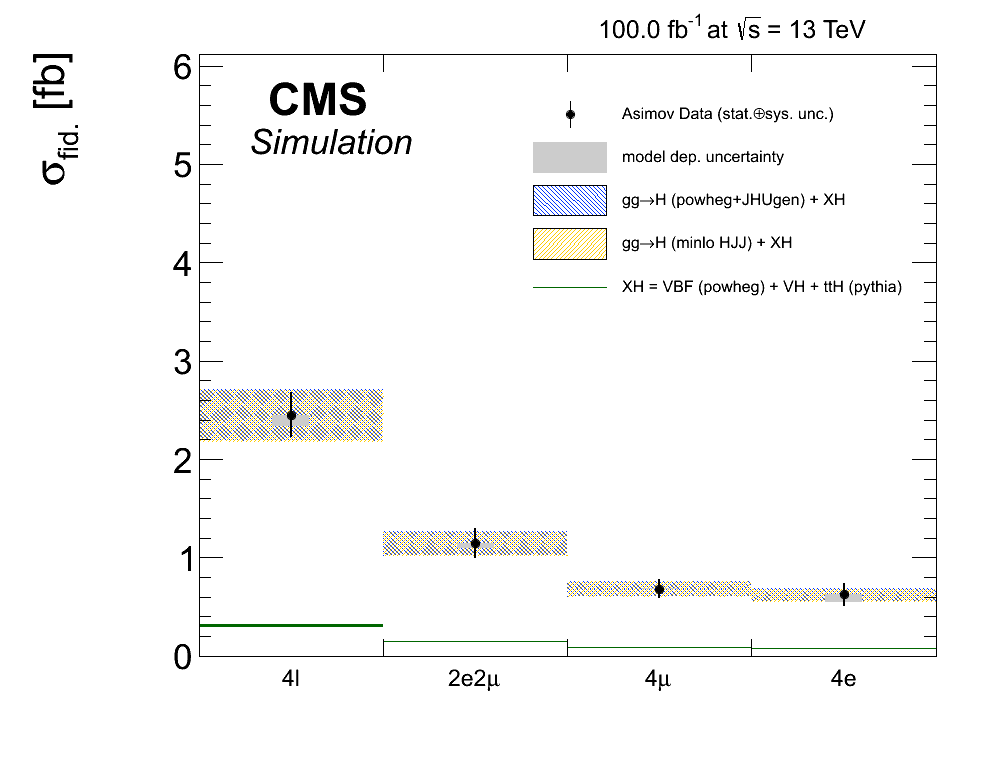
\includegraphics[width=0.65\textwidth,angle=0]{Figures/Higgs_XS_100.png}
      \label{fig:Higgs_XS_100}
    }
    \subfigure[]{
      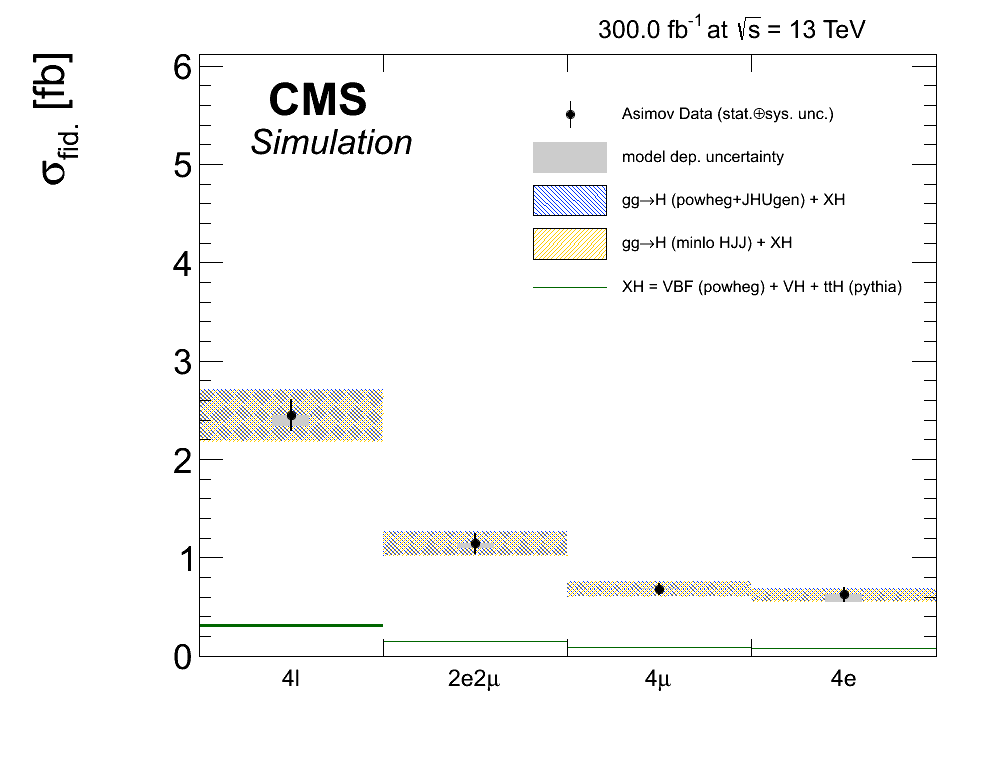
\includegraphics[width=0.65\textwidth,angle=0]{Figures/Higgs_XS_300.png}
      \label{fig:Higgs_XS_300}
    }    
    \caption{ Higgs cross section results using Asimov data corresponding to integrated luminosity of 100~\fbinv(a) and 300~\fbinv at $\sqrt{s} = 13$~TeV 
    along with theoretical predictions per final state.}
  \label{fig:Higgs_XS_100_300}
 \end{center}
\end{figure}